% !TeX root = ../../Book1.tex
% 纲要标题：### 2.1 从仿射图到射影空间
% 纲要位置：几何学计划纲要.md，第 157 行。
% 正文状态：初稿；尚未正式审核。

% 纲要内容开始
% 
% * 一维子空间、齐次坐标与标准仿射图
% * 射影子空间的关联与维数
% * 射影标架及射影变换的唯一确定
% * 射影线上的交比与置换对称
% 
% 纲要内容结束

\section{从仿射图到射影空间}
\label{g1:sec:0201}

在仿射平面中，两条不同直线的关系要分成相交与平行两种。可是从透视图看，平行铁轨似乎也交于远方。射影空间把这种现象变成一个精确的构造：把方向也作为点加入，使平面内任意两条不同直线都有唯一交点。这些方向点将由向量的一维子空间来定义。

\subsection{一维子空间、齐次坐标与标准仿射图}
\label{g1:subsec:0201:01}

本章的基域 \(K\) 为 \(\mathbb R\) 或 \(\mathbb C\)。上一章的仿射组合、基与维数计算也可对复向量空间逐字进行；长度、正负号与正交分类则仍须注明是实 Euclid 结构，不能随之自动推广。

\begin{definition}[射影空间]\label{g1:def:projective-space}
	设 \(K=\mathbb R\) 或 \(\mathbb C\)，\(V\) 是 \(n+1\) 维 \(K\) 向量空间，\(n\geq0\)。以 \(V\) 的一维向量子空间为元素的集合
	\[
		\mathbb P(V)\coloneqq\{Kv:v\in V\setminus\{0\}\}
	\]
	称为 \(V\) 的\term[sheyingkongjian]{射影空间}[projective space]，其射影维数定义为 \(n\)。记 \([v]=Kv\)，并记 \(\mathbb P^n(K)=\mathbb P(K^{n+1})\)。选定 \(V\) 的基后，若 \(v=(X_0,\ldots,X_n)\ne0\)，则 \([X_0:\cdots:X_n]\) 称为该点的\term[qicizuobiao]{齐次坐标}[homogeneous coordinates]。
\end{definition}
\symidx{\(\mathbb P(V)\)：向量空间的一维子空间所成的射影空间}

两个非零向量表示同一点，当且仅当相差一个非零倍数：
\[
	[X_0:\cdots:X_n]=[\lambda X_0:\cdots:\lambda X_n]\qquad(\lambda\in K^\times).
\]
零向量不表示任何射影点。在实数情形，\(v\) 与 \(-v\) 也表示同一点，所以这里取的是过原点的整条直线，并非带方向的射线。\(\mathbb P^0(K)\) 只有一个点，而 \(\mathbb P^1(K)\) 已有无穷多个点。

\begin{proposition}[标准仿射图]\label{g1:prop:projective-charts}
	设 \(K=\mathbb R\) 或 \(\mathbb C\)。对 \(0\leq i\leq n\)，令
	\[
		U_i=\{[X_0:\cdots:X_n]:X_i\ne0\}.
	\]
	映射 \(U_i\rightarrow K^n\) 将一点送到除去第 \(i\) 项后的各个比值 \(X_j/X_i\)，是双射。这些集合覆盖 \(\mathbb P^n(K)\)。在 \(U_i\cap U_k\) 上，若 \(x_j=X_j/X_i\)，并补记 \(x_i=1\)，则第 \(k\) 张图的坐标为 \(y_j=x_j/x_k\)，其中 \(j\ne k\)。
\end{proposition}
\begin{proof}
	同乘非零数不改变任何比值，故映射良定义。反过来，把第 \(i\) 项取为 \(1\)，其余项依次取为所给的 \(n\) 个数，便得到唯一射影点。每个非零向量至少有一个非零分量，所以各图覆盖整个空间。在重叠处 \(x_k\ne0\)，直接相除给出 \(X_j/X_k=(X_j/X_i)/(X_k/X_i)\)，即所述换图公式。
\end{proof}

称 \(U_i\) 为\term[fangshetu]{仿射图}[affine chart]，因为选定归一化 \(X_i=1\) 后它具有通常的仿射坐标。不同图的换图映射一般不是仿射映射。例如在射影线上，\(t=X_0/X_1\) 与 \(s=X_1/X_0\) 满足 \(s=1/t\)。图的用途是让我们在一块区域内使用熟悉的坐标，并明确知道走到另一块区域时如何转换。

\begin{example}[一条射影线中的无穷远点]\label{g1:exm:projective-line}
	在 \(\mathbb P^1(K)\) 中，\(U_1\) 的点唯一写成 \([t:1]\)，余下只有 \([1:0]\)，记作 \(\infty\)。因此作为集合有 \(\mathbb P^1(K)=K\cup\{\infty\}\)。这里的记号不允许直接参与普通实数或复数运算；例如涉及 \(\infty\) 的分式应改用齐次坐标计算。在实数情形，\cref{g1:fig:projective-line-chart}用穿过原点的直线表示这些点。
\end{example}

\begin{figure}[htbp]
	\centering
	% !TeX root = ../Book1.tex
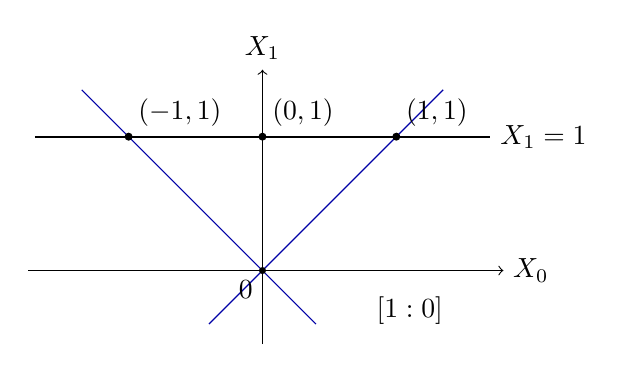
\begin{tikzpicture}[scale=0.85]
	\draw[->] (-3.5,0)--(3.6,0) node[right] {\(X_0\)};
	\draw[->] (0,-1.1)--(0,3) node[above] {\(X_1\)};
	\draw[thick] (-3.4,2)--(3.4,2) node[right] {\(X_1=1\)};
	\draw[blue!65!black] (-0.8,-0.8)--(2.7,2.7);
	\draw[blue!65!black] (0.8,-0.8)--(-2.7,2.7);
	\fill (0,0) circle(1.5pt) node[below left] {\(0\)};
	\foreach \x/\lab in {-2/{(-1,1)},0/{(0,1)},2/{(1,1)}}
	{\fill (\x,2) circle(1.7pt);\node[above right] at (\x,2) {\(\lab\)};}
	\node[below] at (2.2,-0.25) {\([1:0]\)};
\end{tikzpicture}

	\caption[射影线与一张仿射图]{射影线与一张仿射图。与 \(X_1=1\) 相交的每条过原点直线给出一个有限坐标；水平直线 \(X_1=0\) 给出唯一遗漏的射影点 \([1:0]\)。}
	\label{g1:fig:projective-line-chart}
\end{figure}

对 \(\mathbb P^n(K)\)，其中 \(n\geq1\)，选取 \(U_0\)，便把 \(K^n\) 放入射影空间：
\[
	(x_1,\ldots,x_n)\longmapsto[1:x_1:\cdots:x_n].
\]
补集 \(H_\infty=\{X_0=0\}\cong\mathbb P^{n-1}(K)\) 称为这张图的\term[wuqiongyuanchaopingmian]{无穷远超平面}[hyperplane at infinity]。它取决于仿射图的选择，并不是射影空间中预先指定的特殊部分。当 \(n=1\) 时它是一个点；当 \(n=2\) 时是一条射影直线。

\subsection{射影子空间的关联与维数}
\label{g1:subsec:0201:02}

由线性方程定义子空间的办法仍然适用，不过现在方程必须齐次，才能使“是否满足方程”不依赖代表向量。

\begin{definition}[射影子空间]\label{g1:def:projective-subspace}
	设 \(K=\mathbb R\) 或 \(\mathbb C\)，\(V\) 为有限维 \(K\) 向量空间。若 \(W\subseteq V\) 为非零向量子空间，称 \(\mathbb P(W)\subseteq\mathbb P(V)\) 为\term[sheyingzikongjian]{射影子空间}[projective subspace]，维数为 \(\dim_K W-1\)。维数为 \(1\) 的称为\term[sheyingzhixian]{射影直线}[projective line]；余维为 \(1\) 的称为\term[sheyingchaopingmian]{射影超平面}[projective hyperplane]。为统一相交公式，也把空集视为空射影子空间，约定 \(\mathbb P(0)=\varnothing\)，\(\dim\varnothing=-1\)。
\end{definition}

\begin{proposition}[交与张成空间]\label{g1:prop:projective-dimension}
	设 \(K=\mathbb R\) 或 \(\mathbb C\)，\(V\) 为有限维 \(K\) 向量空间，\(U,W\subseteq V\) 为向量子空间，记 \(E=\mathbb P(U)\)、\(F=\mathbb P(W)\)，并约定空射影子空间的维数为 \(-1\)。则 \(\mathbb P(U)\cap\mathbb P(W)=\mathbb P(U\cap W)\)，包含二者的最小射影子空间为 \(\mathbb P(U+W)\)，称为它们的张成空间。若用 \(\langle E,F\rangle\) 表示两个射影子空间的张成空间，则
	\[
		\dim\langle E,F\rangle+\dim(E\cap F)=\dim E+\dim F.
	\]
	特别地，在 \(\mathbb P^n(K)\) 中，\(\dim E+\dim F\geq n\) 蕴含 \(E\cap F\ne\varnothing\)。
\end{proposition}
\begin{proof}
	一个一维空间同时包含于 \(U,W\)，等价于它包含于 \(U\cap W\)，故得交集公式。任何包含 \(\mathbb P(U),\mathbb P(W)\) 的射影子空间，其对应向量空间包含 \(U,W\)，因而包含 \(U+W\)；后者本身也满足包含要求，故为最小者。上一章证明\cref{g1:prop:affine-intersection}时已经通过扩充交集的基得到 \(\dim(U+W)+\dim(U\cap W)=\dim U+\dim W\)。四个维数各减 \(1\)，即得到此处公式，零空间也符合约定。若交集为空，公式给出 \(\dim\langle E,F\rangle=\dim E+\dim F+1\leq n\)，与最后的假设矛盾。
\end{proof}

所以射影平面中两条不同直线恰交于一点：必有交点，而若交空间维数至少为 \(1\)，两条直线就相同。但射影三维空间仍有不相交的直线。例如 \(\mathbb P(\operatorname{span}(e_0,e_1))\) 与 \(\mathbb P(\operatorname{span}(e_2,e_3))\) 不交。加入无穷远点消除了平面内平行线的例外，没有消除高维空间中的异面直线。

\begin{proposition}[仿射子空间的射影补全]\label{g1:prop:affine-projective-completion}
	设 \(K=\mathbb R\) 或 \(\mathbb C\)，\(n\geq1\)，\(F=p+L\subseteq K^n\) 为非空仿射子空间，\(\dim L=d\)。用 \(x\mapsto[1:x]\) 把 \(K^n\) 识别为 \(U_0=\{X_0\ne0\}\subseteq\mathbb P^n(K)\)，并记 \(H_\infty=\{X_0=0\}\)。在此嵌入下，包含 \(F\) 的最小射影子空间为
	\[
		\widehat F=\mathbb P\bigl(K(1,p)+(0,L)\bigr).
	\]
	它具有维数 \(d\)，与 \(U_0\) 的交为 \(F\)，与 \(H_\infty\) 的交为 \(\mathbb P(0,L)\)。
\end{proposition}
\begin{proof}
	所写向量空间包含所有 \((1,p+u)=(1,p)+(0,u)\)，其中 \(u\in L\)。反过来，任何包含这些向量所张成各条直线的向量空间都含 \((1,p)\)，再作差便含全部 \((0,u)\)，故包含所写空间。由于 \((1,p)\notin(0,L)\)，其向量维数为 \(d+1\)。一般向量为 \((a,ap+u)\)：若 \(a\ne0\)，归一化得到 \([1:p+u/a]\)；若 \(a=0\)，得到 \([0:u]\)。这分别给出两种交集。
\end{proof}

\begin{example}[平行线的公共方向点]\label{g1:exm:parallel-infinity}
	在实仿射平面中，两条直线 \(y=0\)、\(y=1\) 的射影补全分别为 \(X_2=0\)、\(X_2=X_0\)。联立可得唯一交点 \([0:1:0]\)，它代表水平方向。一般地，不同平行直线 \(p+Ku\)、\(q+Ku\) 的射影补全都含 \([0:u]\)，而有限部分不交，故交点恰是该方向点。
\end{example}

\subsection{射影标架及射影变换的唯一确定}
\label{g1:subsec:0201:03}

上一章的仿射标架由 \(n+1\) 个点构成，它们唯一确定仿射映射。在射影空间中，每个代表向量还允许独立缩放，所以只指定 \(n+1\) 个独立的点不够；还需要一个点来协调这些缩放。

\begin{definition}[射影变换与射影标架]\label{g1:def:projective-frame}
	设 \(K=\mathbb R\) 或 \(\mathbb C\)，\(V,W\) 是维数相同的有限维 \(K\) 向量空间。可逆线性映射 \(T:V\rightarrow W\) 诱导的双射 \([v]\mapsto[Tv]\) 称为\term[sheyingbianhuan]{射影变换}[projective transformation]，记为 \(\mathbb P(T)\)。在 \(\mathbb P^n(K)\) 中，设 \(n\geq1\)。若一个有序点组的 \(n+2\) 个点 \((p_0,\ldots,p_n,p_*)\) 中，任意 \(n+1\) 个点的代表向量都线性无关，就称这个点组为\term[sheyingbiaojia]{射影标架}[projective frame]。
\end{definition}

这里的射影变换由可逆线性映射诱导。复共轭也保持直线，却涉及基域的自同构，属于不同的变换类别。射影变换把 \(\mathbb P(U)\) 送到 \(\mathbb P(TU)\)，因此保持子空间维数、相交与包含关系。

\begin{theorem}[标架决定射影变换]\label{g1:thm:projective-frame}
	设 \(K=\mathbb R\) 或 \(\mathbb C\)，\(n\geq1\)。任意两个 \(n\) 维射影空间的有序射影标架之间，存在唯一按顺序匹配各点的射影变换。
\end{theorem}
\begin{proof}
	先固定基 \(e_0,\ldots,e_n\)，称 \(([e_0],\ldots,[e_n],[e_0+\cdots+e_n])\) 为标准标架。给定标架，任选 \(p_i\) 的非零代表 \(v_i\)；它们组成基。将 \(p_*\) 的代表写成 \(w=\sum_i a_i v_i\)。每个 \(a_i\ne0\)，否则 \(w\) 与除去 \(v_i\) 的其余 \(n\) 个向量线性相关，违反标架条件。因此线性映射 \(T(e_i)=a_i v_i\) 可逆，且 \(T(\sum_i e_i)=w\)，把标准标架送到给定标架。对另一个标架作同样构造，再将相应映射与前一个映射的逆复合，就得到存在性。

	为证唯一性，只需证明固定标准标架各点的射影变换恒等。其线性代表 \(S\) 固定各坐标直线，故 \(Se_i=c_i e_i\)，其中 \(c_i\ne0\)。又 \([\sum_i c_i e_i]=[\sum_i e_i]\)，由基展开唯一性知所有 \(c_i\) 相同。于是 \(S=cI\)，诱导恒等射影变换。
\end{proof}

同一证明还说明，两个可逆线性映射诱导同一射影变换，当且仅当相差非零标量。因此 \(\mathbb P^n(K)\) 上的射影变换群记为
\[
	\operatorname{PGL}(n+1,K)\coloneqq\operatorname{GL}(n+1,K)/\{cI:c\in K^\times\},
\]
称为\term[sheyingyibanxianxingqun]{射影一般线性群}[projective general linear group]。商掉标量矩阵，把诱导同一射影变换的线性映射归为一类。

\begin{example}[平面标架与分式坐标]\label{g1:exm:projective-frame-map}
	在 \(\mathbb P^2(K)\) 中，取前三点 \([e_0],[e_1],[e_2]\)，再取 \([2:3:1]\)。三个系数非零，所以构成标架。从标准标架到它的变换由 \(\operatorname{diag}(2,3,1)\) 表示。在源、目标都采用 \(X_0\ne0\) 的图时，一般矩阵 \(M=(m_{ij})\) 所诱导的坐标公式为
	\[
		x_i'=
		\frac{m_{i0}+\sum_{j=1}^n m_{ij}x_j}{m_{00}+\sum_{j=1}^n m_{0j}x_j},\qquad i=1,\ldots,n,
	\]
	仅在分母非零的部分成立。分母为零时，射影变换仍有定义，只是像落到目标图的无穷远超平面。例如 \([X_0:X_1:X_2]\mapsto[X_1:X_0:X_2]\) 在 \(x_1\ne0\) 处写成 \((x_1,x_2)\mapsto(1/x_1,x_2/x_1)\)，而 \(x_1=0\) 上的有限点被送到无穷远处。
\end{example}

射影线上的标架就是三个两两不同的点。因此三个指定的不同点可以唯一移到 \(\infty,0,1\)；第四个点在这个归一化之后留下的坐标，就是我们下一步要构造的不变量。

\subsection{射影线上的交比与置换对称}
\label{g1:subsec:0201:04}

线段长之比依赖仿射图，换成分式坐标后通常改变。用四个点形成的适当比值却能把这些变化全部抵消。行列式定义能同时处理有限点与无穷远点。

\begin{definition}[交比]\label{g1:def:cross-ratio}
	设 \(K=\mathbb R\) 或 \(\mathbb C\)，\(A,B,C,D\in\mathbb P^1(K)\) 两两不同，分别取非零代表 \(a,b,c,d\in K^2\)。记 \(\Delta(u,v)=\det(u,v)\)，定义\term[jiaobi]{交比}[cross-ratio]为
	\begin{equation}\label{g1:eq:cross-ratio}
		(A,B;C,D)\coloneqq
		\frac{\Delta(a,c)\Delta(b,d)}{\Delta(a,d)\Delta(b,c)}.
	\end{equation}
\end{definition}

两点不同恰好意味着其代表线性无关，故上述分母非零。每个代表向量的缩放因子在分子分母各出现一次，因而抵消；改变 \(K^2\) 的基又使每个行列式乘以同一非零数，总商仍不变。因此定义也适用于任意二维向量空间的射影线。采用有限坐标 \(A=[a:1]\) 等时，公式成为
\[
	(A,B;C,D)=\frac{(a-c)(b-d)}{(a-d)(b-c)}.
\]
不同书籍有不同的排列约定，比较公式时应先检查哪三个点被归一化为 \(\infty,0,1\)。本书约定满足
\begin{equation}\label{g1:eq:cross-ratio-normalization}
	(\infty,0;1,t)=t.
\end{equation}

\begin{proposition}[有序四点的完全不变量]\label{g1:prop:cross-ratio-orbits}
	设 \(K=\mathbb R\) 或 \(\mathbb C\)，\((A,B,C,D)\) 与 \((A',B',C',D')\) 为 \(\mathbb P^1(K)\) 中两组各自两两不同的有序四点。\(\mathbb P^1(K)\) 的射影自同构保持交比；两组四点可由这样的自同构逐点匹配，当且仅当交比相等，且这个自同构若存在则唯一。交比的取值恰为 \(K\setminus\{0,1\}\)。
\end{proposition}
\begin{proof}
	若变换由 \(T\in\operatorname{GL}(2,K)\) 诱导，则 \(\Delta(Tu,Tv)=\det(T)\Delta(u,v)\)，四个因子抵消，证明不变性。由\cref{g1:thm:projective-frame}，存在唯一变换把前三点变为 \(\infty,0,1\)。第四点不同于前三点，故变为唯一的 \(t\in K\setminus\{0,1\}\)；直接以 \((1,0),(0,1),(1,1),(t,1)\) 代入定义，得到交比等于 \(t\)。于是交比相等的两组四点有同一归一化形式，复合归一化变换便逐点匹配；唯一性仍由前三点决定。反过来，任取 \(t\ne0,1\)，这组标准四点实现所需值。
\end{proof}

\begin{proposition}[置换产生的六种表达式]\label{g1:prop:cross-ratio-permutations}
	设 \(K=\mathbb R\) 或 \(\mathbb C\)，\(A,B,C,D\in\mathbb P^1(K)\) 两两不同，记 \(\lambda=(A,B;C,D)\)。任意重排四点得到的值，都属于下表的六种表达式；表中每种表达式都由所列重排实现，但数值可能重复。


\begin{table}[htbp]
	\centering
	\caption{交比与四点的次序}
	\label{g1:tab:cross-ratio-permutations}
	\begin{tabular}{cccc}
		\toprule
		排列&交比&排列&交比\\
		\midrule
		\((A,B;C,D)\)&\(\lambda\)&\((A,C;D,B)\)&\(1/(1-\lambda)\)\\
		\((A,B;D,C)\)&\(1/\lambda\)&\((A,D;B,C)\)&\((\lambda-1)/\lambda\)\\
		\((A,C;B,D)\)&\(1-\lambda\)&\((A,D;C,B)\)&\(\lambda/(\lambda-1)\)\\
		\bottomrule
	\end{tabular}
\end{table}
\end{proposition}

\begin{proof}
	由不变性可把四点设成 \(\infty,0,1,\lambda\)，代入行列式公式即逐项得到表中各值。还需说明其余排列不会增加新值。交换第一、二个点或第三、四个点，都把当前交比 \(t\) 变为 \(1/t\)；交换第二、三个点则把它变为 \(1-t\)，后者也可在归一化四点上直接计算。任何排列都可通过相邻交换得到：依次把所需的首项移到第一位，再把第二项移到第二位，继续即可。表中的六个分式对 \(t\mapsto1/t\) 与 \(t\mapsto1-t\) 封闭，所以没有其他值。
\end{proof}

\begin{example}[调和四点与次序的影响]\label{g1:exm:harmonic-quadruple}
	交比为 \(-1\) 的有序四点称为\term[tiaohe-sidian]{调和四点}[harmonic quadruple]。例如 \((\infty,0;1,-1)=-1\)，两个有限点 \(1,-1\) 关于 \(0\) 对称。一般地，在实仿射线上 \((\infty,b;c,d)=(b-d)/(b-c)\)，所以等于 \(-1\) 恰好意味着 \(b=(c+d)/2\)。“中点”本身依赖所选无穷远点，而四点构成的射影关系不依赖图。对于 \(\lambda=-1\)，\cref{g1:tab:cross-ratio-permutations}的六式只有 \(-1,2,1/2\) 三个不同值，说明交换次序可以保留同一无序点集，却改变交比。
\end{example}

于是，标架把位置选择中的自由度固定下来，交比记录仍未消除的参数。这个“先归一化，再读出不变量”的步骤将在圆锥曲线的参数与六点构造中再次使用。
